\documentclass[]{scrreprt}
\usepackage[utf8]{inputenc} 
\usepackage{graphicx}
\usepackage{pdfpages}
\usepackage{tabularx}
\usepackage{cite} 
\usepackage{caption}
\usepackage{todonotes}

\usepackage{glossaries} 

\usepackage{hyperref}
\hypersetup{
	colorlinks=true,        % false: boxed links; true: colored links
	linkcolor=black,        % color of internal links
	%    citecolor=green,        % color of links to bibliography
	citecolor=black,        % color of links to bibliography
	filecolor=magenta,      % color of file links
	urlcolor=blue           % color of external links
}


% Title Page
\title{Comparison of different machine learning algorithms for music genre classification\\ \tiny ..with some of them containing methods that could be remotely seen as "visualization"}
\subtitle{GitHub: https://github.com/SinForest/iaml-project}
\author{Patrick Dammann (3144913) \and Florian Fallenbüchel (3144974) \and Thorsten Wünsche (3148266)}

\begin{document}
\maketitle

\begin{abstract}
\end{abstract}

\tableofcontents

\chapter{Introduction}
by Patrick Dammann

\bigskip

The automated analysis of music is an expanding field, mainly because of the increasing popularity of music streaming services. Since these companies usually earn money through monthly subscriptions and can only minimally compete through their product range, they have to satisfy their customers with features and comfort.

One highly demanded feature is a good song recommendation, since it is hard for people to find new music they like, especially in the sheer infinite amount of music most services offer. This is where modern machine learning approaches can shine, since good recommendation needs good analysis of the listeners, as well as the music they are listening to.

Here, genre classification comes into account. While the main results of the successful training of a genre-classification-model might not be very helpful in this terms, finished models can be used to extract features that can give an abstract and numerical interpretation of songs to improve future analysis of the musical tastes of individuals to help them finding new music to listen to.

Aside from capitalistic motivations, this project was also designed to get better insights on how neural networks work on music data, since it is handled very differently from common data like images, texts and even sound data containing speech.

\section{Outlook}

This project will discuss several methods for music genre classification. First, we explain how our dataset is made up, to then directly try an approach that uses convolutional neural networks on the raw sample data. The following approach combines complicated, hand-crafted features with a simple, fully-connected neural network. The last method utilizes frequency-based preprocessing together with a convolutional and recurrent neural network.
\chapter{Dataset}\label{dataset}
\textit{by Florian Fallenbüchel}\\

The dataset which we will use in our experiments consists of 106574
songs, downloaded from the Free Music Archive~\cite{fma_dataset}. This
gives us 917 GB of Creative Commons-licensed audiofiles, tagged with the
respective genres. While a song may have multiple subgenres from a range
of 161 genres, the data set assigns a single top genre to each song. We
will use these top genres as labels in our experiments. There are 16
different top genres in the data, while some songs have tagged an empty
string.

\section{Distribution of the genres}

Figure~\ref{unfiltered} shows the genre distribution over the
full data set. Unfortunately, we realized too late, that the empty genre
is considered a class, and therefore, that the data is heavily
imbalanced. This influenced most of the experiments we did with the set,
delivering 53$\%$ accuracy for some of our neural networks, which only
predicted the empty genre. The individual chapters will provide more
insight.
\begin{figure}[!htb]
	\centering
	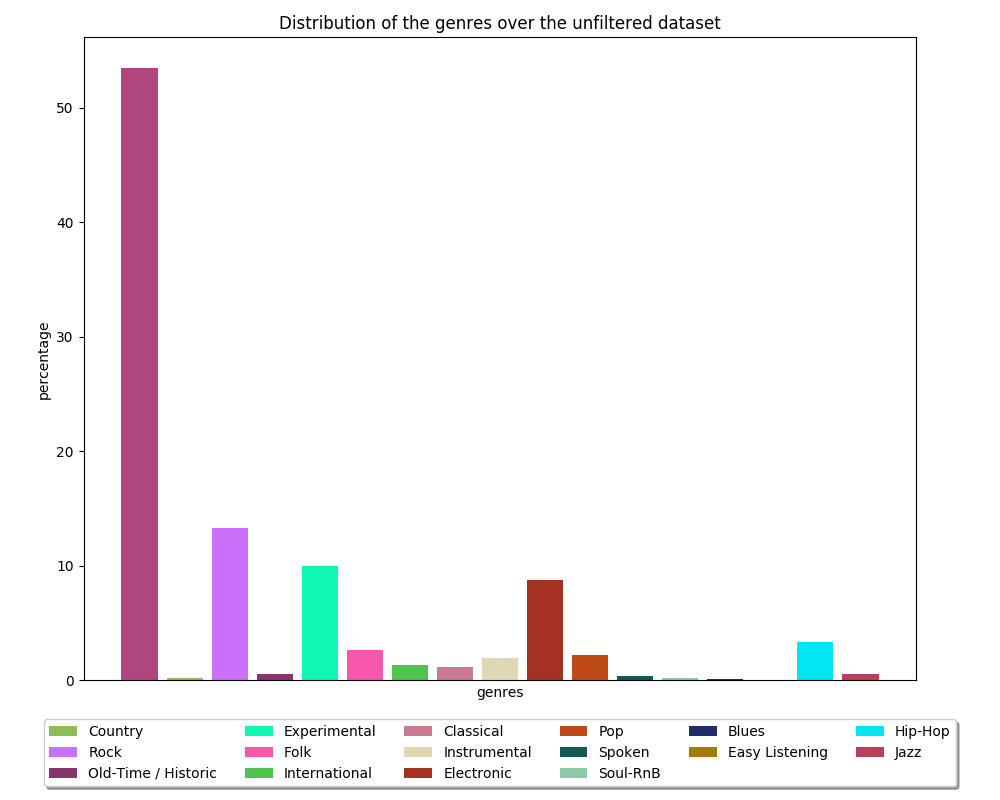
\includegraphics[width=0.9\textwidth]{images/genredist.png}
	\caption{Distribution of the genres over the dataset.
	About 53$\%$ of the data (left bar) has no top genre tagged.}
	\label{unfiltered}
\end{figure}

Therefore, we had to filter the songs from the set which were untagged,
as they hinder training not only by delivering high accuracy for the
prediction of a single class, but also, because the songs are probably
from one of the other 16 classes in reality and therefore have similar
features to the remaining songs, but a different tag. This leaves us
with 49598 songs from the original set. Figure~\ref{filtered} pictures
the distribution of the genres after the tracks with no top genre got
filtered out. As you can see, the data is still imbalanced, with a
majority of the songs being either Rock, Experimental or Electronic
music. To improve results in the future, we should filter out genres
with small sample sizes. Due to the deadline, we were only able to redo
some of our tests we already carried out on the full dataset.\\
\begin{figure}
	\centering
	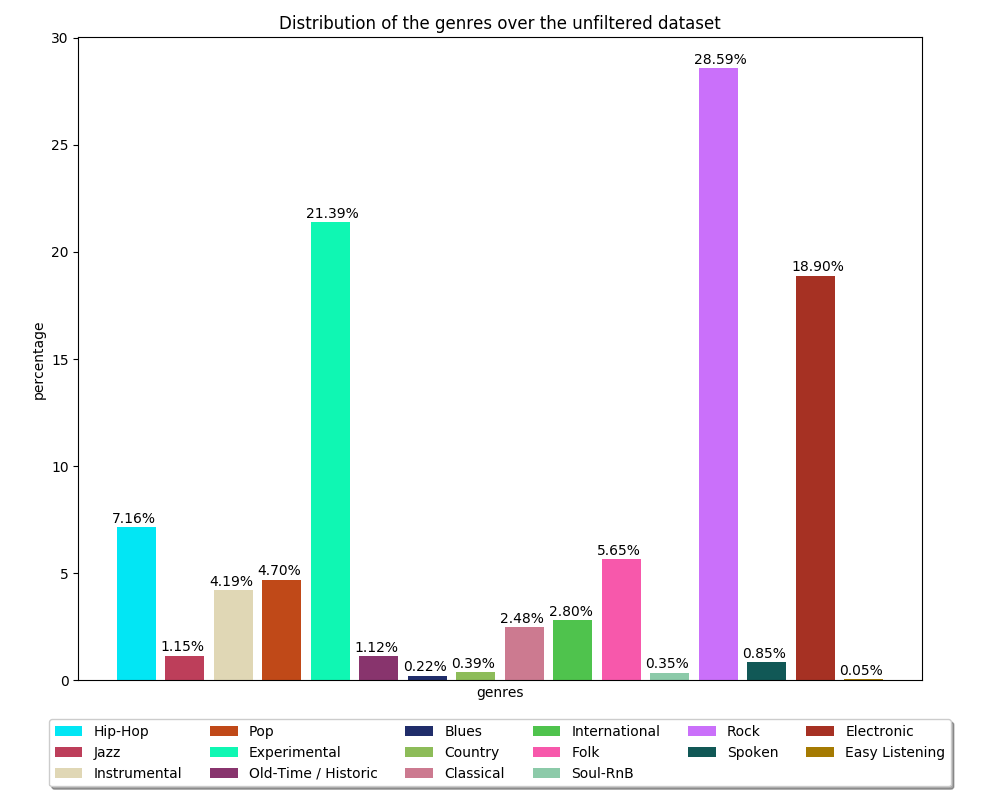
\includegraphics[width=0.9\textwidth]{images/genredistfiltered.png}
	\caption{Distribution of the genres over the filtered dataset with no empty
	top genre.}	
	\label{filtered}
\end{figure}
We used 20\% of our data for testing, resulting in 39679 songs for
training and 9919 for validation (85260 and 21314 in the unfiltered data
set). As the dataset has an ordering of genres, due to tracks of the
same album usually being the same genre, we shuffle the data before
splitting to obtain a similar distribution over the two sets.
Figure~\ref{trainval} shows the genre distributions of our filtered
train and validation sets. As you can see, the genres are indeed equally
distributed for the two sets, but the classes themself are still
imbalanced. The distribution of the splits for the experiments carried
out with the unfilterd data set also follow the distribution of the
whole data in Figure~\ref{unfiltered}. This should be taking into
account while evaluating our accuracy statistics.

\begin{figure}
	\centering
	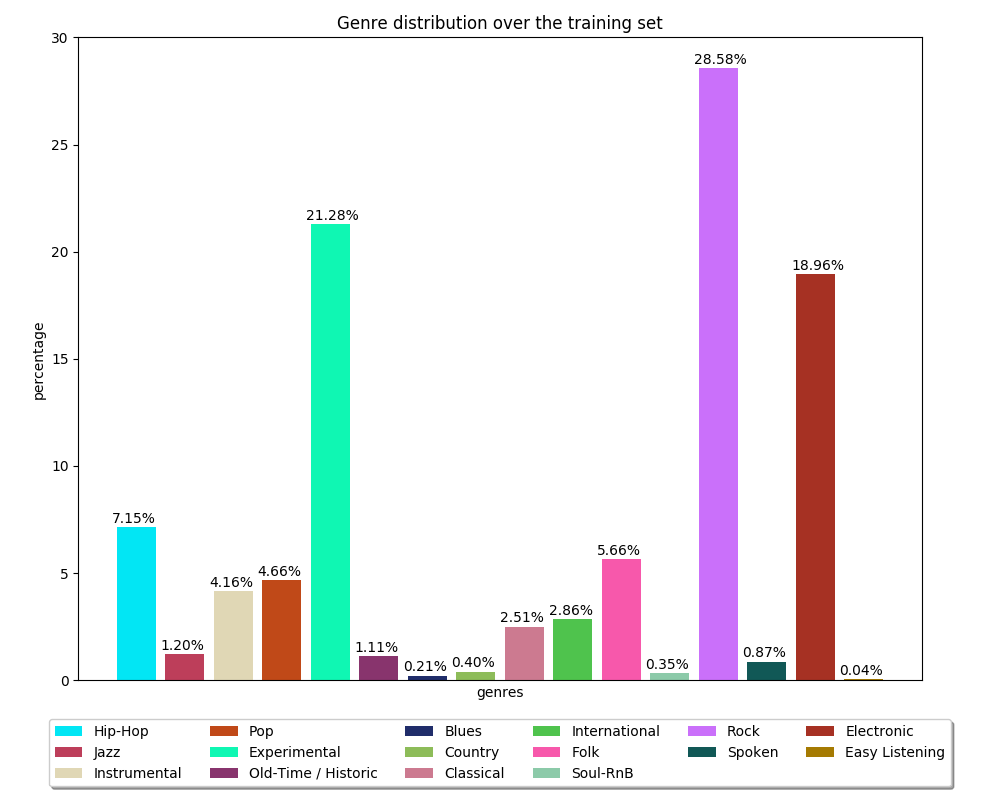
\includegraphics[width=1.0\textwidth]{images/train.png}
	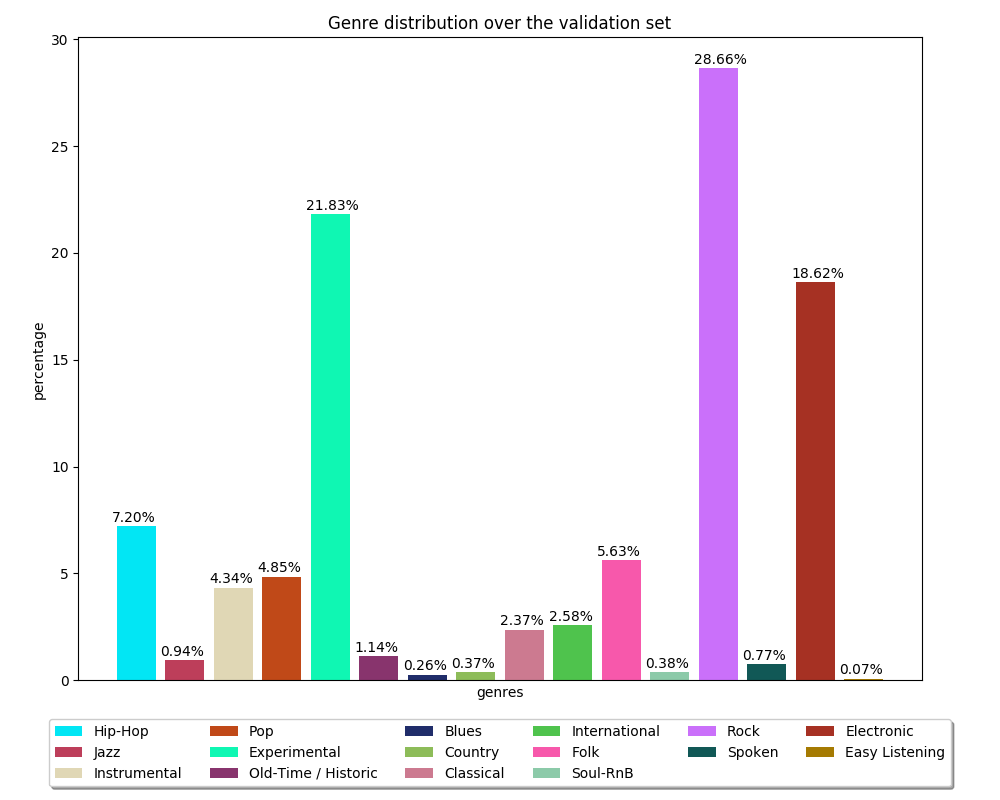
\includegraphics[width=1.0\textwidth]{images/val.png}
	\caption{Genre distribution over the training and validation
	sets. The two distributions are quite similar.}
	\label{trainval}
\end{figure}
\chapter{Sample-level CNN using raw waveforms}
\textit{by Thorsten Wünsche}\\

In this chapter, we attempt to recreate an approach that reduces preprocessing by working with raw waveforms directly in a deep convolutional neural network. 

Section \ref{sec:theory} presents the original paper. In section \ref{sec:development}, we discuss the development process up until the first working prototype. Experiments and improvements to our own version are described in section \ref{sec:experiments}. Finally, section \ref{sec:conclusion} summarizes our experiences with this approach.

\section{Theory and original paper}
\label{sec:theory}
The paper "Sample-level Deep Convolutional Neural Networks for Music Auto-tagging Using Raw Waveforms" \cite{DBLP:journals/corr/LeePKN17} by Jongpil Lee, Jiyoung Park, Keunhyoung Luke Kim and Juhan Nam suggests an approach that works with raw waveforms directly. This differentiates it from our other models, which pre-compute entropy and MEL spectograms respectively.

Not only does this approach use raw waveforms, it also examines this data a few samples at a time, making it equivalent to pixel-level or character level when working with images and text respectively. 

Their suggested model consists of an initial convolution layer with equal filter length and stride, which combines a small number of samples into frames. These are then passed through $n$ convolution layer with filter length $m$ and stride one, each followed by a max-pooling layer with stride $m$. Each stage also makes use of batch-normalization and a ReLU activation function. Finally, the net ends with a fully connected layer with a $0.5$ dropout chance and a sigmoid output layer.

To allow for small values for both n and m (below 15), the input must be a short part of the song, between one and four seconds. The sample length of these tracks must be equal, as the dimensions of the model depend on it. The average of several segments is then used as the prediction.

After experimenting with different values for $m$ and $n$ as well as segment length, their most successful model uses $m=3$, $n=9$ and a segment length of 2678 ms at 22050 Hz. The structure of their model is shown in table \ref{tab:sample-dcnn_original-model}. For their learning rate, 0.01 is used as the initial value, reducing by a factor five after three consecutive epochs, in which the validation loss did not decrease. Training was halted while the learning rate was at 0.000016.

\begin{center}
	\begin{tabular}{ c c c c}
		
		layer & stride & output & \# of params\\
		\hline
		\hline
		conv 3-128 & 3 & 19683 x 128 & 512 \\
		\hline
		conv 3-128 & 1 & 19683 x 128 & 49280 \\
		maxpool 3 & 3 & 6561 x 128 & \\
		\hline
		conv 3-128 & 1 & 6561 x 128 & 49280 \\
		maxpool 3 & 3 & 2187 x 128 & \\
		\hline
		conv 3-256 & 1 & 2187 x 128 & 98560 \\
		maxpool 3 & 3 & 729 x 256 & \\
		\hline
		conv 3-256 & 1 & 729 x 256 & 196864 \\
		maxpool 3 & 3 & 243 x 256 & \\
		\hline
		conv 3-256 & 1 & 243 x 256 & 196864 \\
		maxpool 3 & 3 & 81 x 256 & \\
		\hline
		conv 3-256 & 1 & 81 x 256 & 196864 \\
		maxpool 3 & 3 & 27 x 256 & \\
		\hline
		conv 3-256 & 1 & 27 x 256 & 196864 \\
		maxpool 3 & 3 & 9 x 256 & \\
		\hline
		conv 3-256 & 1 & 9 x 256 & 196864 \\
		maxpool 3 & 3 & 3 x 256 & \\
		\hline
		conv 3-512 & 1 & 3 x 512 & 393728 \\
		maxpool 3 & 3 & 1 x 512 & \\
		\hline
		conv 1-512 & 1 & 1 x 512 & 262656 \\
		dropout 0.5 & - & 1 x 512 & \\
		\hline
		sigmoid & - & 50 & 25650 \\
		
		& & & \\	
	\end{tabular}
	\label{tab:sample-dcnn_original-model}
	\captionof{table}{The original model with the parameters Jongpil Lee, Jiyoung Park, Keunhyoung Luke Kim and Juhan Nam found to be the most successful. The layer "conv3-128 maxpool3" is to be understood as a one dimansional convolutio layer with filter length 3 producing 128 filters, followed by a maxpool layer with pooling length 3. The 50 in the sigmoid layer is the number of labels in the dataset (both MSD and MTAT, using the 50 most common tags).}
\end{center}


\section{Development and limitations}
\label{sec:development}

\begin{figure}[!htb]
	\centering
	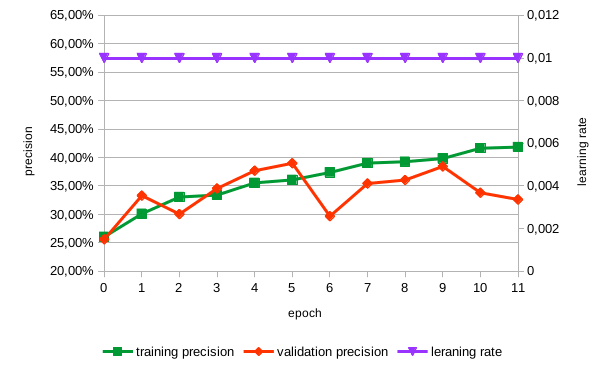
\includegraphics[width=.9\linewidth]{images/sample-dcnn-m3-n9-seg10-128_512-plateau.png}
	\caption{Performance of the $3^9$ model using 10 segments of music, between 128 and 512 filters and a reduce on plateau learning rate with the parameters suggested in the paper.}
	\label{fig:sample-dcnn-m3-n9-seg10-128_512-plateau}
\end{figure}


We created our own prototype by recreating the most successful model found by Jongpil Lee, Jiyoung Park, Keunhyoung Luke Kim and Juhan Nam. Their $3^9$ model shown in table \ref{tab:sample-dcnn_original-model} uses a one dimensional filter of size three in a convolutional neural network of depth 9 (1+9+1).  Using a frame-size of three, this model converts 59049 samples into 19683 frames. We also use the same sample rate (22050 Hz), so that each input into the model covers 2678 ms of audio.

The large FMA dataset \cite{fma_dataset} would not only take far too long to train on a desktop computer, but is also too large to be stored on the available hard drives. Therefore we use the small version of the dataset with 8000 songs (30 s each) distributed evenly across 8 top-level genres to adjust our model, before we attempt to classify the larger version on a server. Some of the files in the small dataset are corrupt or too short. Where not enough data for our model is available, the tensors are filled up with random numbers between - 1 and 1. As the defect files are in the single digits, this should not have a noticeable effect on the performance.

The performance of our initial implementation is shown in figure \ref{fig:sample-dcnn-m3-n9-seg10-128_512-plateau}. The learning rate scheduler does not seem to work as intended and possibly due to a constant learning rate of $0.01$, the accuracy leaves a lot to be desired. Even with these limitations, the model reaches an accuracy of 25\% on both the training and the validation set after a single epoch. In a balanced dataset with eight classes, this is already twice as good as a naive approach. The precision on both sets rises by 10-15 percentage points, though the validation precision declines soon after. All in all, this prototype works, but will need to be adapted to our hardware and time limitations.


\section{Experiments}
\label{sec:experiments}

Next, we will tweak the prototype described in section \ref{sec:development}. This will involve changing hyper-parameters as well as the filter-length and depth of the model. Using a CPU with eight virtual cores and a GeForce GTX 1060 6GB, the training of the prototype completed 12 epochs within eight hours. The following experiments are limited to this same timespan. This does mean that the model may not fully converge, but our primary concern is finding modifications that can increase the performance of our model before training it on the larger dataset using more capable hardware. 

\subsection{Learning rate}

\label{subsec:learning_rate}
\begin{figure}[!htb]
	\centering
	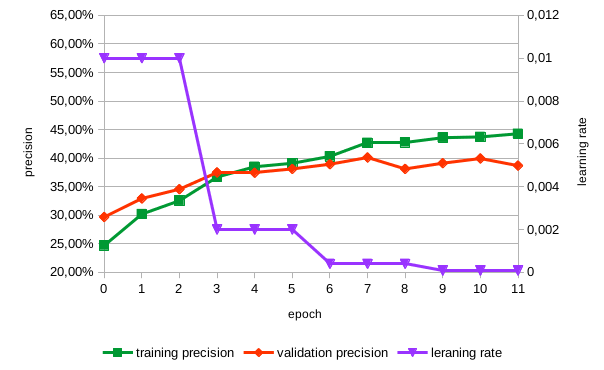
\includegraphics[width=.9\linewidth]{images/sample-dcnn-m3-n9-seg10-128_512-step.png}
	\caption{Performance of the $3^9$ model using 10 segments of music and between 128 and 512 filters. This version was modified to use a step learning rate dividing by a factor five every three epochs.}
	\label{fig:sample-dcnn-m3-n9-seg10-128_512-step}
\end{figure}

The first subject of experimentation is the learning rate. In the original prototype, we use the same model as Jongpil Lee, Jiyoung Park, Keunhyoung Luke Kim and Juhan Nam: The learning rate starts at $0.01$ and decreases by a factor five when the validation loss has not decreased in three consecutive epochs. In eight hours of training on a desktop computer, our prototype finished 12 epochs. This means that a quarter of the total training time would be required to identify a plateau. Indeed, during our initial training the learning rate was not reduced even once. With more time or faster hardware, this would be acceptable. We want to conduct a few other experiments as well however, and therefore tried two other approaches.

First, we keep the starting rate of $0.01$ and reduce it by the same factor five after three epochs regardless of the validation loss. This leads to three decreases over the course of one session. In the paper, training was halted after four decreases.

As can be seen in figure \ref{fig:sample-dcnn-m3-n9-seg10-128_512-step}, the accuracy on the validation set with our modification not only rises above 40\% at one point, it also remains much more stable, making it an overall improvement. The downside of this approach is, that after a few more epochs, the learning rate will be too low to allow for further improvement, even if the model and the dataset still had potential. As we plan to also apply our model to a larger dataset on more powerful hardware, this schedule might prove too limiting.

To adjust the learning rate in a more flexible manner, we return to the reduce on plateau scheduler, but make some adjustments to allow it to be effective even with limited time and hardware. We reduce the patience period from three to zero, reducing immediately upon a rise in the validation loss. As this makes the scheduler more vulnerable to small mistakes, we reduce the factor of the division from five to two and add a one epoch cooldown, to give the validation loss time to recover after the learning rate has been reduced.

The results are shown in figure \ref{fig:sample-dcnn-m3-n9-seg10-128_512-plateau_mod}. The validation accuracy is initially less stable, but ends up at similar values to the previous experiment, while the precision on the training set rises to above 50\%. Most importantly, this scheduler adapts itself to the dataset and slows down only when required, rather than at a constant and possibly too high speed.

We conclude, that our modified version of the reduce on plateau scheduler is an improvement on our limited hardware and will use this version in all experiments from here on out. On more powerful hardware however, the original version will likely be superior, as it is less susceptible to small fluctuations in the validation loss.


\begin{figure}[!htb]
	\centering
	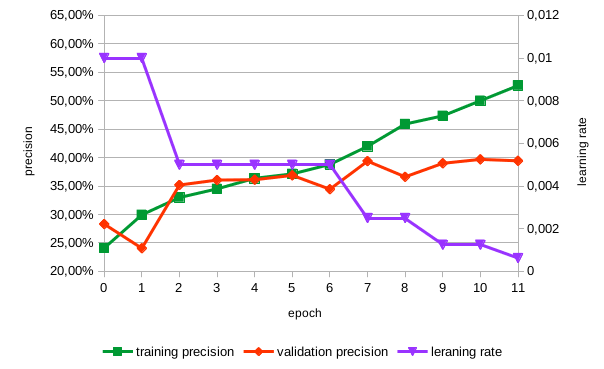
\includegraphics[width=.9\linewidth]{images/sample-dcnn-m3-n9-seg10-128_512-plateau_mod.png}
	\caption{Performance of the $3^9$ model using 10 segments of music and between 128 and 512 filters. This version was modified to use a reduce on plateau learning rate dividing by a factor 2 after every epoch, in which the validation loss did not fall. After every reduction, there is a one epoch cooldown to give the loss a chance to recover.}
	\label{fig:sample-dcnn-m3-n9-seg10-128_512-plateau_mod}
\end{figure}


\subsection{Number of filters}

In the paper, the authors experiment both on MTAT and MSD. For MTAT, increasing the number of filters in the convolution layers from 16 to 512 was sufficient, but performance on MDS improves when starting at 128 filters. Our prototype uses 128-512 filters initially, in this experiment, we reduce the number of filters in the earlier layers to 16 and gradually raise the number to 512. If this method results in a reduced training time without sacrificing accuracy, then the increased number of epochs may make up for the somewhat lower complexity.

\begin{figure}[!htb]
	\centering
	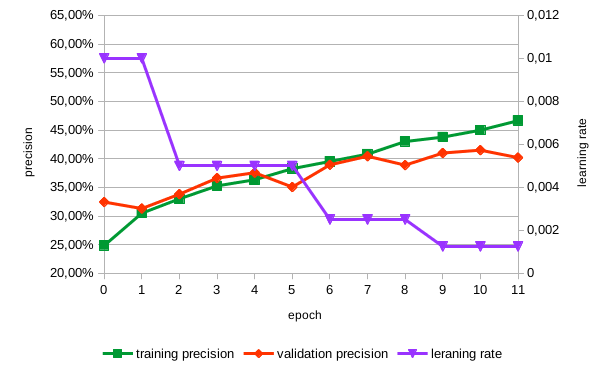
\includegraphics[width=.9\linewidth]{images/sample-dcnn-m3-n9-seg10-16_512-plateau_mod.png}
	\caption{Performance of the $3^9$ model using 10 segments of music and the modified reduce on plateau learning rate described in subsection \ref{subsec:learning_rate}. This version uses a reduced number of filters, increasing from 16 to 512 rather than 128 to 512.}
	\label{fig:sample-dcnn-m3-n9-seg10-16_512-plateau_mod}
\end{figure}

After training the model for eight hours, no significant decrease in training time was found. As shown in figure \ref{fig:sample-dcnn-m3-n9-seg10-16_512-plateau_mod}, the accuracy on the validation set however grew slightly, while the training precision fell significantly. This would suggest, that our previous model was overfitting to a small degree. Therefore we will keep using the reduced number of filters on the small dataset (8000 samples), but will increase it back to full for more complex applications.

\subsection{Number of segments}
\label{subsec:segments}

All models up to now have used ten segments of music, all of equal length, and averaged over the  results. We now reduce the amount of segments to one, hoping to achieve an increase in training speed without sacrificing too much accuracy.

\begin{figure}[!htb]
	\centering
	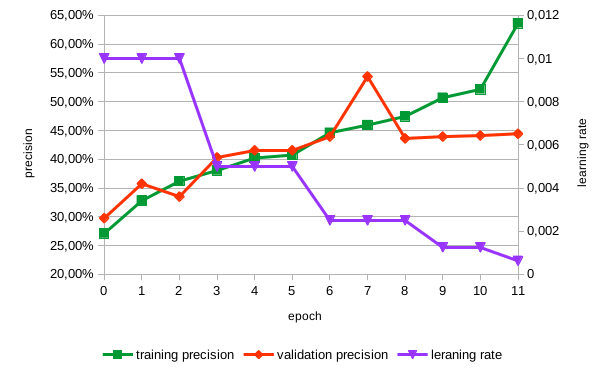
\includegraphics[width=.9\linewidth]{images/sample-dcnn-m3-n9-seg1-16_512-plateau_mod.png}
	\caption{Performance of the $3^9$ model using the modified reduce on plateau learning rate and a reduced number of filters, increasing from 16 to 512 rather than 128 to 512. This Version trains and classifies only one segment of music at a time.}
	\label{fig:sample-dcnn-m3-n9-seg1-16_512-plateau_mod}
\end{figure}

Figure \ref{fig:sample-dcnn-m3-n9-seg1-16_512-plateau_mod} shows, that this modification is very effective, reducing the time needed to train and evaluate one epoch on the small dataset from 43 minutes to only twelve. The reduced training time is most likely due to having the dataloader handle only three instead of 30 seconds of music. In our current system, the CPU is clearly the bottleneck and this change lightens the load, allowing the GPU to receive data quicker. Due to leaving the model training overnight, the total time spent is a bit longer than the initial eight hours. This allows for significantly more epochs, which in turn increases the validation accuracy by 5\% compared to all previous models. In the later epochs the training and validation accuracy are almost equal.

\begin{figure}[!htb]
	\centering
	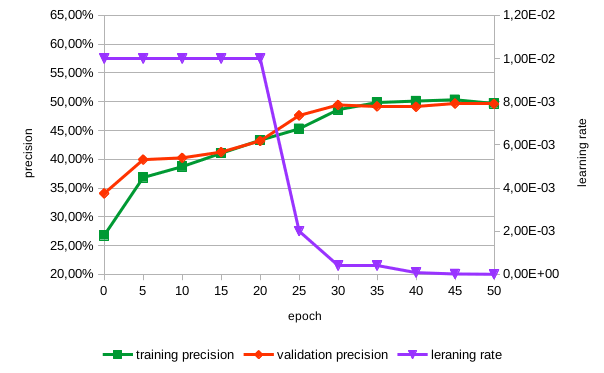
\includegraphics[width=.9\linewidth]{images/sample-dcnn-m3-n9-seg1-128_512-plateau.png}
	\caption{Performance of the first $3^9$ model using only one segment of music instead of ten.}
	\label{fig:sample-dcnn-m3-n9-seg1-128_512-plateau}
\end{figure}

The higher number of epochs also requires a reconsideration of the learning rate scheduler. In subsection \ref{subsec:learning_rate} we concluded that the original scheduler was too slow for our format. As the number of epochs can now realistically be quintupled, we return to the original settings, with only the number of segments reduced from ten to one. Figure \ref{fig:sample-dcnn-m3-n9-seg1-128_512-plateau} shows, that we were right to do so: Compared to the prevoius experiment, both training and validation accuracy increase by another 5\%, since the learning rate in the later epochs is not too small to prevent improvement. After epoch 46, the scheduler reduces the learning rate the fifth time, at which point Jongpil Lee, Jiyoung Park, Keunhyoung Luke Kim and Juhan Nam considered the training complete.

As the original model is now outperforms the other versions, we return to the full 128-512 filters and the reduce on plateau learning rate scheduler, which reduces after three epochs with no improvement to the validation loss.

\subsection{Depth and filter length}

We wanted to try changing the dimensions of the model in at least one experiment. Originally, a $3^6$ model was planned, hoping to reduce the training time. Now that subsection \ref{subsec:segments} has shown, that the CPU is our bottleneck, reducing the training time is no longer likely. We will instead train this model to find out how much of a difference the lower number of layers makes. If the depth can be reduced without lowering the accuracy significantly, this would make the model more suitable to being used on less powerful devices after the training is complete. 



\begin{figure}[!htb]
	\centering
	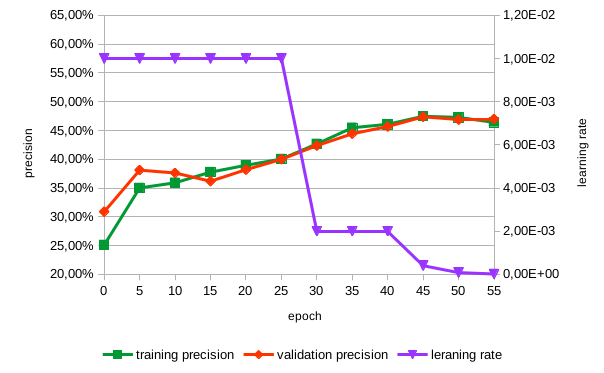
\includegraphics[width=.9\linewidth]{images/sample-dcnn-m3-n6-seg1-128_512-plateau.png}
	\caption{Performance of the $3^{6}$ model using one segment of music (2678 ms), the original reduce on plateau learning rate scheduler and 128-512 filters.}
	\label{fig:sample-dcnn-m3-n6-seg1-128_512-plateau}
\end{figure}

In figure \ref{fig:sample-dcnn-m3-n6-seg1-128_512-plateau}, we can see that the $3^{6}$ model reaches accuracy of about 3 percentage points under the $3^{9}$ version and requires more epochs to train. This may be very useful when applying the pre-trained model to weaker hardware, such as mobile devices, as the lower depth allows for faster classification. The lack of depth would likely cause significantly worse performance on more complex datasets.

To take advantage of the GPU power, which is currently going unused, we also train a deeper version. This new model uses 1+14+1 layers and a filter length and step size of 2. This model will not be able to use the same segments as our other versions, so we reduce the segment length to 32768 samples (1486 ms).

\begin{figure}[!htb]
	\centering
	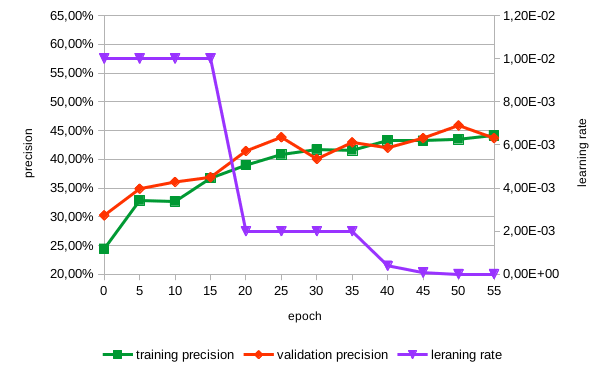
\includegraphics[width=.9\linewidth]{images/sample-dcnn-m2-n14-seg1-128_512-plateau.png}
	\caption{Performance of the $2^{14}$ model using one segment of music (1486 ms), the original reduce on plateau learning rate scheduler and 128-512 filters.}
	\label{fig:sample-dcnn-m2-n14-seg1-128_512-plateau}
\end{figure}

Figure \ref{fig:sample-dcnn-m2-n14-seg1-128_512-plateau} shows, that the  $2^{14}$ model requires more epochs to train than the  $3^{9}$ model, likely due to the added depth. The accuracy however is lower for both the training and validation set. This may be caused by the smaller filter, which requires a significantly higher number of layers to process longer inputs.

\section{Conclusion}
\label{sec:conclusion}

We were able to implement the model described in "Sample-level Deep Convolutional Neural Networks for Music Auto-tagging Using Raw Waveforms" \cite{DBLP:journals/corr/LeePKN17} and achieve a training and validation accuracy of 50\% on the small FMA dataset \cite{fma_dataset} within about ten hours on a desktop computer.

While we originally planned to train the best-performing model from the previous experiments on a server with the full dataset, this regrettably failed. The full set contains a number of files, that our dataset class was unable to load. These failures seemed to occur randomly, but frequently enough that training was not possible. As we found this problem fairly late in the project and both other team-members could use preprocessed data, thus bypassing this problem, we decided to use the remaining time to train the other two model using the more powerful hardware.

This approach is slow to train, since it requires large inputs, which have to be reloaded in each epoch. This puts a significant burden on the CPU, even if a powerful GPU is available.
Once the model is trained however, using it for predictions is fairly straight-forward. It can make reasonable predictions even with a small trainingset and using less than four seconds at a 22050 Hz sample rate. By making multiple predictions per song using different segments, misleading parts of a track can be overcome. Furthermore, by choosing segments at random during training, each song effectively can function as multiple different samples. The lack of pre-processing also makes this method suitable to being used on less powerful devices once the model has been trained.
\chapter{Entropy and Fractal Dimension Approach}
\textit{by Florian Fallenbüchel}\\
This chapter will explain our approach on the classification of the
genre via the entropy and fractal dimension of the song. This approach
is interesting, because it does not consider musical information such as
harmony, melody, beat and tempo, heavily reducing the size of the data
to be processed during training. The entropy is a measure of the
disorder of the signal, indicating the quantity of change of the signal
energy between consecutive parts of the track. The fractal dimension is
a measure of the complexity of the signal, as it indicates the ratio of
the change of detail to the change in scale at which the detail is
measured. This term is mostly used in fractal geometry, as fractals have
infinite lengths between any two points, making them more complex than
their topological dimension, but less complex than the next higher one.
This interdimensionality is given by the fractal dimension.\\

\section{Method}
We follow the work of Goulart \textit{et al.}~\cite{entropy} from 2012,
who used the entropy approach together with combined support vector
machines. They achieved 100\% classification accuracy on a set of 90
songs equally distributed over 3 different genres, with 80-90\% of the
data used for training. We try to extend this method to a larger amount
of classes, combining it with neural networks for classification.\\
For the calculation of the entropy, we need the energy approach of
signal theory, as presented in Elements of Information Theory
\cite{infotheo} by Cover and Thomas. The song is divided into frames of
1024 samples with 50\% overlap between consecutive frames and the
entropy $E$ then is defined as
\begin{equation}
	E = - \sum_{i=0}^{1023} p_{i} \log_{2}(p_{i}),
\end{equation}
with $p_{i}$ being the proportion of the sample energy to the
energy of the whole frame
\begin{equation}
	p_i = \frac{y_i}{\sum_{j=0}^{1023} y_j}.
\end{equation}
\\
\noindent From the now obtained set of entropies of the song we
calculate five features, namely the average entropy, the standard
deviation of the entropies, the maximum and minimum entropy and the
absolute maximum difference of entropies between consecutive frames.
Those are the first five entries of our input vector for the neural
network.\\
For the calculation of the fractal dimension they suggest a box counting
algorithm. The basic principle of these algorithms is to calculate the
number of boxes of different sizes necessary to cover the entire signal.
After that, a linear least squares solution is computed on the logarithm
of the number of boxes and the inverse logarithm of the respective box
size ($\frac{1}{log(boxs)}$). The slope of the resulting curve then
resembles the fractal dimension.\\
For the implementation of the algorithm, we needed to improvise, because
the box counting algorithm Goulart \textit{et al.} used in their work is
described in the book ``Fractal Speech Processin''~\cite{fractal} by
Al-Akaidi, which is not purchasable or accessible through online
libraries at the moment. We therefore adopted the box counting algorithm
presented by Boshoff~\cite{boxcount}, as it promises fast computation
time due to the doubling of the box size during each step. The fractal
dimension is the last element of our input, resulting in a six
dimensional input vector for the neural network. We vectorized all
algorithms, to be able to efficiently process the huge amount of
available data in a short amount of time.

\section{Model}
As our input data is relatively simple, we can use a conservative
implementation of a neural network for the classification, without the
need for convolutions. Figure~\ref{entropymodel} shows the architecture
of our naive network design. Our hidden layers are of size 1024 and we
chose parameterized ReLUs with a parameter for every connection, as well
as batch normalization and dropout for every layer. Batch normalization
accellerates training, as it reduces the amount by what the hidden unit
values shift around, normalizing the input from previous layers to a
common scale. The dropout layers should stabilize the prediction
accuracy by eliminating parts of the information during training,
reinforcing the remaining neurons.

\begin{figure}
	\centering
	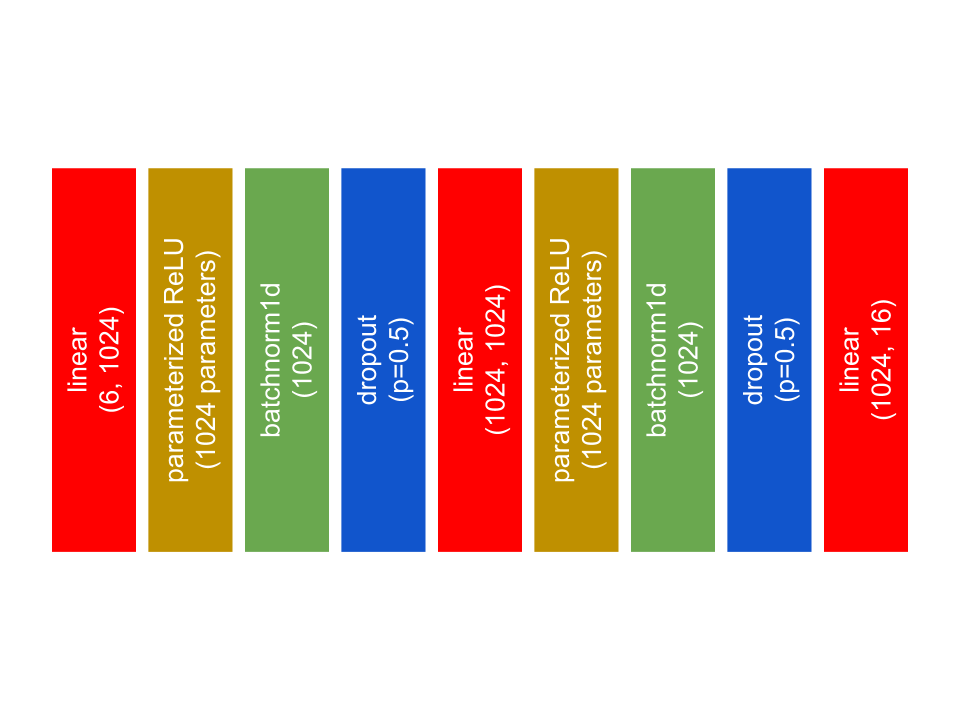
\includegraphics[width=0.65\textwidth]{images/entropymodel.png}
	\caption{Architecture of the neural network used for the classification
	of the 6-dimensional entropy-fractal vector to one of the 16 top
	genres from the dataset.}
	\label{entropymodel}
\end{figure}

\section{Training}
For the training, we used a maximum of 180 seconds per song, as processing
the full length of every track would have taken several days on our
available hardware.

\begin{center}
	\begin{tabular}{ p{0.25\textwidth} p{0.2\textwidth} p{0.2\textwidth} p{0.2\textwidth}}
		Genre & Accuracy & Hits & from Total\\
		\hline
		Instrumental & $0.00\%$ & 0 & 430\\
		Folk & $0.00\%$ & 0 & 558\\
		Country & $0.00\%$ & 0 & 37\\
		Pop & $0.00\%$ & 0 & 481\\
		Hip-Hop & $8.54\%$ & 61 & 714\\
		Electronic & $52.52\%$ & 970 & 1847\\
		International & $0.00\%$ & 0 & 256\\
		Rock & $78.29\%$ & 2226 & 2843\\
		Spoken & $0.00\%$ & 0 & 76\\
		Blues & $0.00\%$ & 0 & 26\\
		Old Time / Historic & $5.31\%$ & 6 & 113\\
		Easy Listening & $0.00\%$ & 0 & 7\\
		Experimental & $45.87\%$ & 993 & 2165\\
		Classical & $34.04\%$ & 80 & 235\\
		Jazz & $0.00\%$ & 0 & 93\\
		Soul-RnB & $0.00\%$ & 0 & 38\\
	\end{tabular}
		\label{tab:accperclass}
	\captionof{table}{Accuracy per class after 100 epochs of training with the filtered data set.}
	\end{center}
\def\code#1{\mbox{\texttt{#1}}}


\chapter{Recurrent Convolutional Neural Network}
\textit{by Patrick Dammann}

\bigskip

This chapter of the project will focus on an attempt using a model, that combines convolutional layers followed by a recurrent layer with preprocessing based on fourier transformation.

\section{Related Work}
\label{sec:rcnn-related}
The model used in this chapter was proposed by a blog post
\footnote{http://deepsound.io/music\_genre\_recognition.html}
by DeepSound, where they used it on the GTZAN \cite{1021072} dataset. Here, we try to adapt their method and applying that model to a bigger dataset.

The main idea of the model is based on convolutional neural networks (where it is hard to choose any the right papers to mention), and LSTMs \cite{Hochreiter:1997:LSM:1246443.1246450}, which are a special form of recurrent layers.

A blog post \footnote{http://benanne.github.io/2014/08/05/spotify-cnns.html} by a spotify intern uses a similar approach.

\section{Mel Spectrograms / Preprocessing}
\label{sec:rcnn-mels}

This approaches main attempt was to analyse sound in a similar way to humans. Since we humans perceive sounds as individual tones, but then give them a new meaning when they are combined in the right way, at the same time as well as in a sequence. Our hearing uses cells, that perform a frequency decomposition: this can easily be simulated via a discrete fourier transformation, since our data is present in discrete data points. To be able to analyze individual or consecutive tones, we need to analyze short, overlapping windows of the music to be sure that things that humans would consider a single sound is caught. This technique is called the Short Time Fourier Transform (STFT), which does a fourier transformation for each sliding window. The paper assumes that the shortest, distinguishable sound is about 10ms long, which would be near to $2048$ samples at $22050$Hz sampling rate(~0.0929ms), so we use this as the window size, while using $1024$ as the stride, to enforce an overlap of $50\%$ between two adjacent windows.

\begin{minipage}{1.0\textwidth}
\[
    stft(m, \omega)=\sum^{\infty}_{n=-\infty}s[n]w[n-m]e^{-i \omega n}
\]
\[
    x := \text{sampled signal}
\]
\[
    w := \text{window function, that is $1$ for selected window, $0$ otherwise}
\]
\vspace{1cm}
\end{minipage}

\begin{figure}
    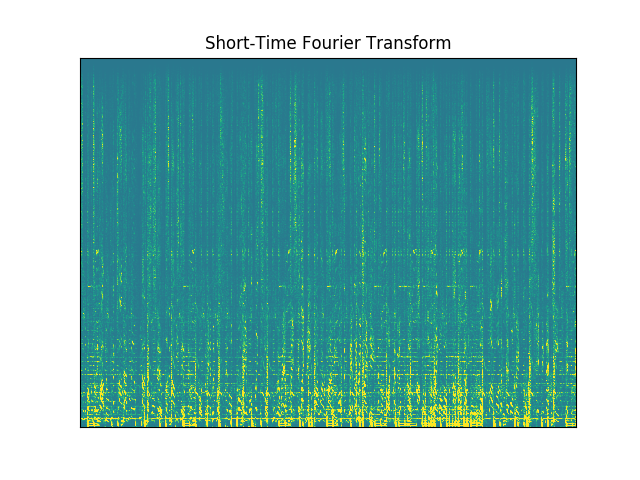
\includegraphics[width=0.5\textwidth]{{images/pepe/stft}.png}
    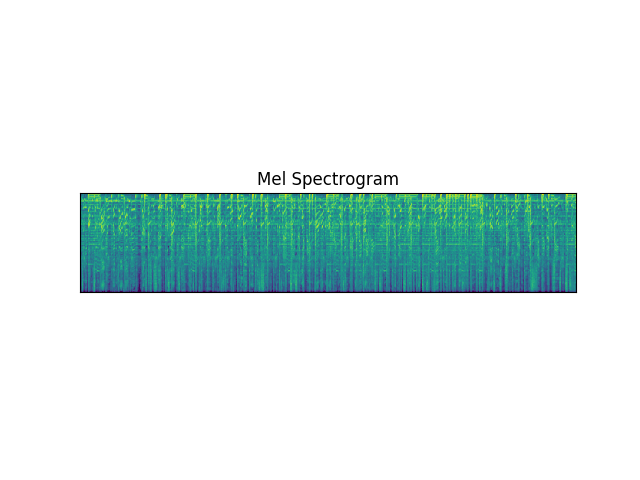
\includegraphics[width=0.5\textwidth]{{images/pepe/mel}.png}
\caption{\label{fig:rcnn-mels}Here, we see the difference between the Short-Time Fourier Transformation (\emph{left}) and the Mel spectrogram (\emph{right}). Primary, the difference in the dimensionality (through the binning) can be seen immediately, while the other advantages are not to be spotted by the naked eye. Both visualizations have in common that they plot the frequency domain on the y-axis and the time domain on the x-axis.}
\end{figure}


A Mel spectrogram is basically the same thing, but converts frequencies to Mel scale (a unit that tries to map equal distances to tones, that humans perceive as equally distanced), and then sums them up to a given number of bins.
We use $128$ bins for our spectrogram, since the hearable spectrum ranges from ~16HZ to  ~19,000Hz, which are $~10.2$ octaves, which are $~123$ tones, so we should be catching everything that gathers around the "main frequencies in the traditional tone ladder" as a single feature.

An optical comparison between the two is provided in figure \ref{fig:rcnn-mels}.

\section{The Model}
\label{sec:rcnn-model}

\begin{figure}
    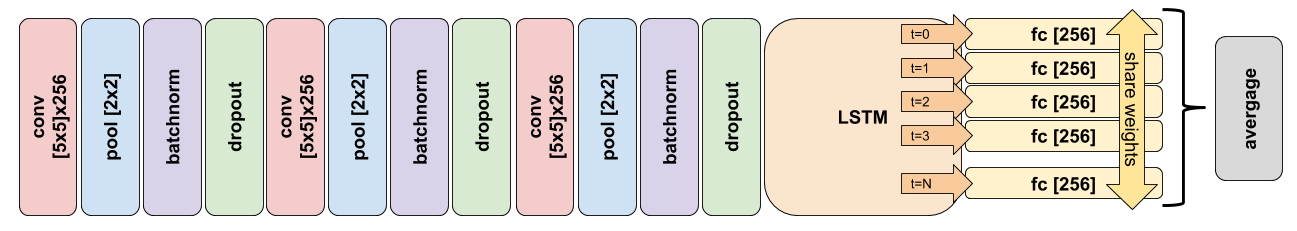
\includegraphics[width=1.0\textwidth]{{images/pepe/model}.png}
\caption{\label{fig:rcnn-model}This is the used model architecture. The model starts with it's convolutional layers (together with their usual companions), followed by an LSTM and a time-distributed fully connected layer, over whose scores is averaged unweighted.}
\end{figure}

The first part of the network consists of convolutional layers. Since tones in all frequencies can be combined to create a hearing experience, it makes sense to consider the frequency domain as feature axis, so the \mbox{\texttt{Conv1D}} layers' filters are two-dimensional and shifted along a single axis, the time axis. This way, information about different frequency bins can be combined over a short amount of time in each laver. Around the convolutional layers, which utilize \code{ReLU} activations, there are \code{BatchNorm}, \code{Pooling} and \code{Dropout} layers.
A visualization of the model can be seen in figure \ref{fig:fig:rcnn-model}.

The next part is a \mbox{\texttt{LSTM}}, which is a special form of a recurrent layer. LSTM cells carry a state and have several weight matrices that, dependent on state and input, give out instructions on how to alter the state as well as an output.
Therefore, LSTMs are used to analyze sequences, since the state allows them to combine information over very long signals and to treat features differently dependent on their predecessors. This is why we then feed the individual feature vectors for each discrete time step into the LSTM, and apply a fully connected layer to the output of each. This fully connected layer has the same weights for each time step.
DeepSound argue that e.g. a rock song should sound like a rock song at every part of the song. Another reason why this might be a good idea is that this way, the gradient should vanish a lot less during backpropagation, since each step in the LSTM is considered for the final result. 

\section{Initial Pre-Processing}
\label{sec:rcnn-pre-proc}
Since the dataset is huge and the song's durations vary strongly, random crops of the song were used, which have been turned into mel spectrograms by the \emph{pytorch} \mbox{\texttt{Dataloader}} on demand. During this approach, training epochs have needed too much time to train many of them, which is why benchmarks of the proportion of data preprocessing time to training time have been made.
Based on these measurements and the opinion that the gain in time is definitely worth the additional needed space, all data is then pre-processed by a script before training, which creates mel spectrograms for all full songs and saves them on hard disk. During training, files are loaded from disk and cropped randomly with a fixed size along the time axis. 

\section{First Training}
\label{sec:rcnn-first}

\begin{figure}
    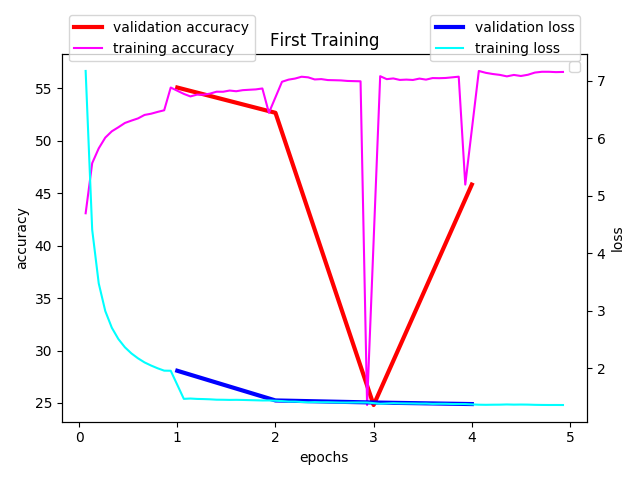
\includegraphics[width=0.5\textwidth]{{images/pepe/logs1.p}.png}
    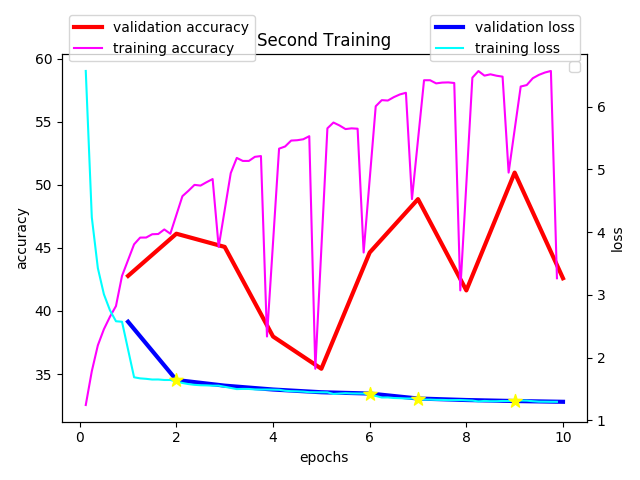
\includegraphics[width=0.5\textwidth]{{images/pepe/logs2.p}.png}
    \caption{\label{fig:rcnn-train} On the left, one can see the training progress of the first session. The validation accuracy is not stable at all and does not reach anywhere near acceptable results. The training has been canceled early.\\
    On the right, the second session is plotted. The validation accuracy seems a lot more stable than before, which might be thanks to the filtered dataset. The yellow stars denote a reduction of the learning rate to one third.}
\end{figure}

The first training was continued over $4$ to $5$ epochs, but then canceled, since we found problems with the data, as mentioned in chapter \ref{dataset}. Like in all following training sessions, \code{RMSprop} with its default configuration has been used as optimizer.
The data shown in figure \ref{fig:rcnn-train} is included to show the difference to further training sessions.
With $~53.5$\% of the songs that seems to belong to all different kinds of genres being labeled with no label, the best achieved accuracy of $~55$\% is only slightly better than always guessing "no label".

\section{Second Training}
\label{sec:rcnn-second}
This training session has been made with the filtered dataset, where all songs without label have been removed. The validation accuracy here peaks at $~50$\%, which is better than the $~55$\% of the previous attempt, considering the structure of the dataset, but still worse than the $70+$\% achieved in the paper\footnote{But, they are only using $10$ genres instead of $16$}. We believe, that the unlabeled data in the dataset "confused" the network by training it to assign the empty label to songs, that should actually be categorized into on the other classes.

\section{Third Training}
\label{sec:rcnn-third}

\begin{figure}
    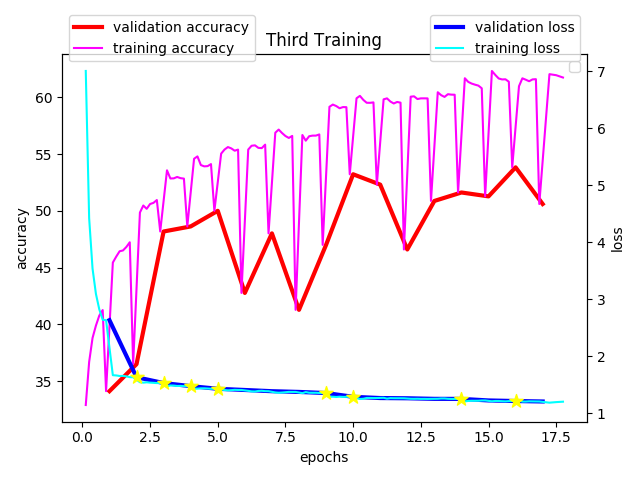
\includegraphics[width=0.7\textwidth]{{images/pepe/logs3.p}.png}
    \caption{\label{fig:rcnn-train2} This session showed the so far most stable and best accuracies and losses achieved during the third training session, with $~53$\% peak accuracy on the filtered dataset.}
\end{figure}

In a follow-up experiment, the performance was tried to be improved by Xavier/2 weight initialization\cite{pmlr-v9-glorot10a} and longer training time. The model itself has not been altered. The results have been plotted into figure \ref{fig:rcnn-train2}.

\section{Including a Visualizing Bottleneck}
\label{sec:rcnn-gen}

\begin{figure}
    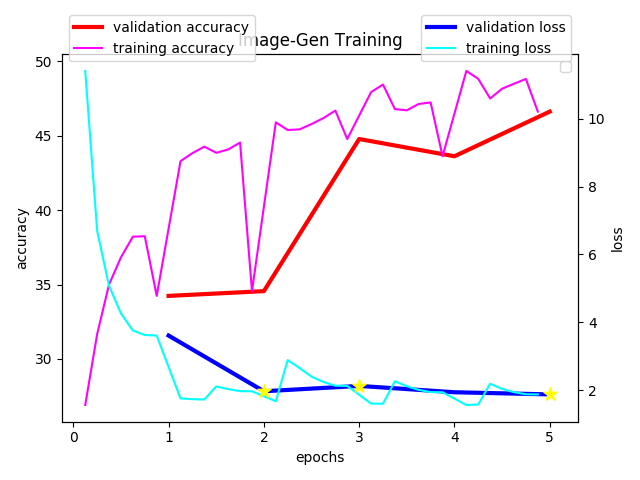
\includegraphics[width=0.45\textwidth]{{images/pepe/logs4.p}.png}
    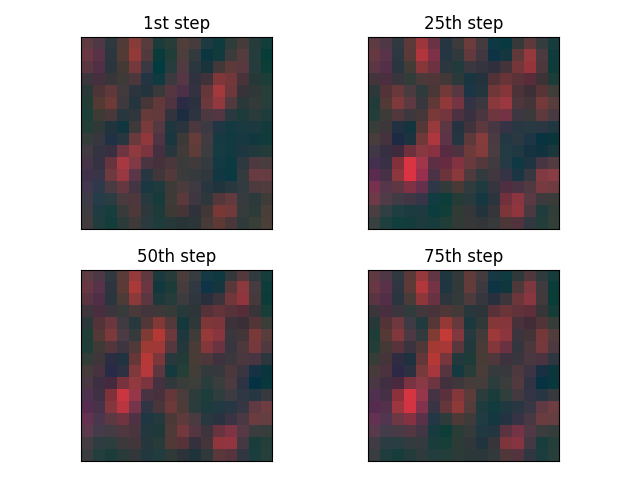
\includegraphics[width=0.25\textwidth]{{images/pepe/image_gen_1}.png}
    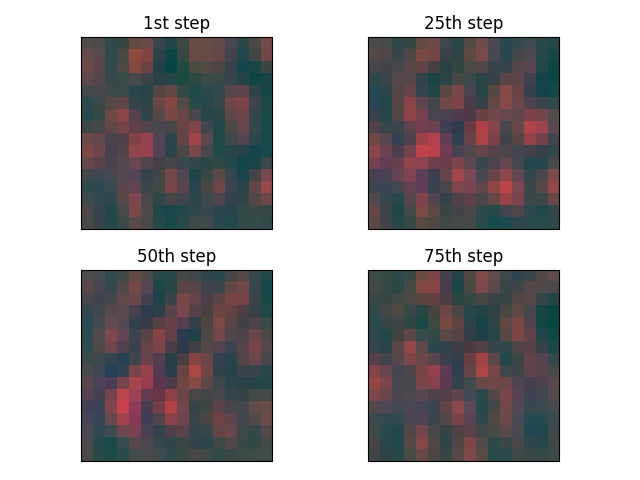
\includegraphics[width=0.25\textwidth]{{images/pepe/image_gen_2}.png}
    \caption{\label{fig:rcnn-gen} The training session on the altered model went well, what the stable accuracy in the left plot shows. Yellow stars are again indicating a scheduling of the learning rate.\\
    On the right are images sampled from two different rock songs. While small differences can be seen, the main hot spots appear at the same places. Unfortunately, all values resolved around zero before the tanh, which is why these images have been mostly grey and had to be boosted in contrast to be viewable and representable with 24bit color depth.}
\end{figure}

Out of interest, the following step was to alter the model in a way that it would not only classify music, but also be able to generate visualizations for music that resembles it in a way learned by the model. The approach taken here to achieve this is to add time-distributed convolutional layers between the LSTM and the time-distributed linear layers, that would create something that could be resembled as an image. Realizing this was easy by reshaping the outputs of the LSTM to squares with shape $16x16$ and then applying convolutional layers with only three filter banks to them. Afterwards, the resulting "image" is additionally blurred with a gaussian filter to make the image look less aliased by decreasing difference and increasing dependence between adjacent pixels.\\
When a visualization is about to be extracted from the network, the song is put in and for each time step the resulting image is returned. For being able to interpret the result as an image, an additional tanh-layer is applied, so all values lie between $0$ and $1$.\\
Adding the image generation layers did not decrease accuracy much, but definitely notable, with a new maximum of $~46.5$\%, but the stability of the validation accuracy suggests that more epochs could have generated better results. An example for visualizations generated by the model can be seen in figure \ref{fig:rcnn-gen}, together with a plot of the training process.

\section{Future Improvements}
\label{sec:rcnn-future}

While the first attempts failed miserably, the latter attempts might have gained good performance through longer training time and a more balanced (and therefore less biassed) dataset. The generation of images in the middle of the network could definitely be improved by some means. Things to test out in the future might involve better post processing, producing a more image-like look and feel through an additional loss on the image instead of a simple blur or more feature maps in the time-distributed convolutional layers of the network, so it can fnd more features in that data that has "seen" all of the song.
\chapter{Conclusion}
by Patrick Dammann

\bigskip

In this project, several methods for music genre classification have been tested. While the first part focussed on handling the raw signal of the song with a specially designed neural network, the following two parts concentrated on good preprocessing and models that are designed to handle it.

Since the dataset was heavily imbalanced, our results can't be directly compared, for accuracies up to $~68$\% can be achieved by ignoring $13$ of the $16$ genres completely. The imbalance of the dataset therefore also heavily influenced our training, since a high bias on frequent labels should be the easiest and most promising direction for the network to follow to obtain low losses. In the end that also means that our results are not very meaningful.

\section{Future Attempts}
First and foremost, future research need a more structured dataset. Since we wanted to perform better than previous attempts on this problem, one of our initial intents was to use more data, which seemed to be simple with the enormous dataset we found. Being way to enthusiastic about the dataset we forgot to check whether there could be errors in it, since it seemed to be well preprocessed by its offerers. With the empty label removed from the beginning, we could have saved much time on unnecessary work and trainings.

The imbalance of the dataset turned out to be a way bigger problem than we initially thought. While we first thought about the bias in the set as a wanted bias, since a big archive like the FMA might resemble the real-world-distribution of music, we soon learned that out models mainly concentrated on learning a bias than on learning general classification qualities.

With a new dataset, other improvements could be realized. For example, the combination of individual models. Especially the pre-processed data of the entropy attempt can easily be fed into another network, maybe helping it by erasing the need to generate similar features itself or by boosting classification by adding a dimension where the data can be more easily separated.

Also, we often copied and sometimes guessed hyper-parameters. These could have been optimized via gaussian processes, or more advanced algorithms like the one provided by \emph{pytorch} used for the entropy approach.
Unfortunately, these optimizations cost a great amount of time for networks with a higher forward- and backward-pass time and of course a higher number of hyper-parameters.
%% Bibliography
% natbib style, requires the usage of natbib: \bibliographystyle{plainnat}
\bibliographystyle{alpha}
\bibliography{literature}%Bibliography file name

%\listoffigures

%\listoftables

\end{document}          
